\section{Ablations: what the design needs}
\label{sec:ablations}
The ablations remove one element of Algorithm~\ref{alg:jpc} at a time and read the result against the reason \S\ref{sec:joint} gave for it.

\paragraph{The critic must move with the policy.}
Figure~\ref{fig:frozen} shows the failure that~(\ref{eq:biasm}) predicts for a critic that is not refitted. With the critic frozen at its pre-trained weights, the pathwise update helps for 500 iterations on Game24 ($+3.4$ at 250, $+3.1$ at 500) and then finds the critic's blind spots: between iterations 500 and 800 the critic's value on the training batch climbs from $\approx3$ to $\approx90$ while the true success rate of the same batch falls to zero, and held-out accuracy falls to $2.1$ at 750. The identical run with two head steps per actor step on the replay buffer keeps the value in the calibrated range and reaches $+15.7$ (Table~\ref{tab:g24_abl}). One head step per actor step lags from 750 iterations on; eight match two; a buffer of 4k states matches 16k.

\paragraph{One chain.}
A policy trained under the cheap $\gamma4$@16 chain improves that chain by $+7.1$ but ends nine points below the deployment-trained policies at the deployment sampler (Table~\ref{tab:g24_abl}, last rows): the value, and with it the improvement, belongs to the chain it was defined on, which is why Algorithm~\ref{alg:jpc} trains under the sampler that will be deployed and why \S\ref{sec:loop} is needed for the others.

\paragraph{Which states the critic learns from.}
The head is refitted on the state at the top of the window only. An earlier version of the recipe stored five evenly spaced steps of the window instead. On Countdown, where the pre-trained critic's held-out AUC is $0.64$ at steps $8$--$24$ of 64 and $0.90$ at step 40, fitting the early states cost the 2D critic three points ($46.9/46.0/47.5$ against $50.1/50.2/50.4$ over three seeds), while on Sudoku, K\&K and Game24 the two versions agree within a point ($70.0/79.2/58.9$ against $71.0/79.6/58.8$). The pre-training of the copy is the other lever. On K\&K, with Algorithm~\ref{alg:jpc} otherwise unchanged (five-step buffer), a critic pre-trained on 16k rollouts at five stored steps for six epochs gives $71.2/72.0/70.6$ and collapses by 500 iterations; the same critic pre-trained on 32k rollouts at seven steps for ten epochs gives $79.5/79.1/79.0$. The pooled value's correlation with the outcome barely changed between the two ($0.70$ against $0.71$ on held-out rollouts), but the correlation of the minimum per-position value rose from $0.38$ to $0.66$: the actor uses the field, not only its mean. The same budget did not change the other tasks, whose critics were already sharp (Appendix~\ref{app:details}).

\paragraph{Step size.}
At an actor learning rate of $3\times10^{-6}$ the 2D critic reaches the level of Table~\ref{tab:main} within 250 iterations and then collapses, on Countdown from $50.1$ to $28.5$ and on Game24 from $58.0$ to $30.3$ by iteration 1000; the scalar critic at the same rate is seed-fragile (Appendix~\ref{app:lr_regime}). At $10^{-6}$ every 2D run of Table~\ref{tab:main} holds, and with the cosine decay none declines before its last checkpoint. The bias~(\ref{eq:biasm}) is paid per step, and the step is the one setting that separates a run that holds from one that collapses.

\paragraph{The rest changes speed, not level.}
With the pooled loss term alone, or without the AUC safeguard, single Game24 runs reach $59.0$ and $58.7$ against $58.9$ for the full recipe but sit $2$--$4$ points lower at 500 iterations (Appendix~\ref{app:details}).

\begin{figure}[t]
\centering
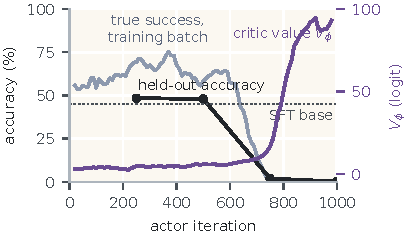
\includegraphics[width=0.9\linewidth]{figures/fig_frozen.pdf}
\caption{Frozen against jointly trained critic on Game24 (2D critic, $10^{-6}$). Red: the critic's value on the training batch; grey: the true success rate of that batch; blue: held-out accuracy at the deployment sampler. With a frozen critic the value is driven to $\approx90$ while success collapses to zero; with the head refitted after every actor step the value stays calibrated and the policy improves.}
\label{fig:frozen}
\end{figure}

\begin{table}[t]
\centering\small
\caption{Game24 ablations of joint training (2D critic, $10^{-6}$): held-out accuracy at $\gamma56$@64 by iteration (base $45.0$) and ODE-64 accuracy at the best checkpoint (base $35.2$). Reference row: mean of three seeds; other rows: single runs. The last two rows are one run trained under $\gamma4$@16, read at two samplers.}
\label{tab:g24_abl}
\resizebox{\linewidth}{!}{%
\begin{tabular}{@{}lccccc@{}}
\toprule
variant & @250 & @500 & @750 & @1000 & ODE-64 (best) \\
\midrule
frozen critic (no refit) & 48.4 & 48.0 & \phantom{0}2.1 & \phantom{0}0.3 & 38.0 \\
critic steps $m_{\rm c}{=}1$ & 48.0 & 51.7 & 48.6 & 51.1 & 40.3 \\
critic steps $m_{\rm c}{=}8$ & 47.0 & 52.3 & 54.7 & 55.2 & 40.5 \\
buffer $N_{\mathcal B}{=}4$k & 47.8 & 50.1 & 52.6 & 56.4 & 42.4 \\
trained under $\gamma4$@16, read at $\gamma56$@64 & 44.7 & 44.3 & 41.5 & 47.0 & 36.7 \\
trained under $\gamma4$@16, read at $\gamma4$@16 & 35.1 & 38.7 & 41.3 & 42.5 & --- \\
\midrule
\hl{Algorithm~\ref{alg:jpc} ($m_{\rm c}{=}2$, $N_{\mathcal B}{=}16$k, deployment chain)} & 48.7 & 50.9 & 53.0 & 56.4 & 42.0 \\
\bottomrule
\end{tabular}}
\end{table}
